\documentclass[conference]{IEEEtran}
\IEEEoverridecommandlockouts
% The preceding line is only needed to identify funding in the first footnote. If that is unneeded, please comment it out.
\usepackage{cite}
\usepackage{mathtools} 
\usepackage{stackengine}
\def\delequal{\mathrel{\ensurestackMath{\stackon[1pt]{=}{\scriptstyle\Delta}}}}
\usepackage{amsmath,amssymb,amsfonts}
\usepackage{amsmath,epsfig,cite,amsfonts,amssymb,psfrag,subfig}
\usepackage{graphicx}
\usepackage{textcomp}
\usepackage{xcolor}
\usepackage{algorithm}
\usepackage[noend]{algpseudocode}
\usepackage{amsthm}
\def\BibTeX{{\rm B\kern-.05em{\sc i\kern-.025em b}\kern-.08em
    T\kern-.1667em\lower.7ex\hbox{E}\kern-.125emX}}
\allowdisplaybreaks
\newtheorem{remark}{Remark}
\newtheorem{theorem}{Theorem}
\newtheorem{lemma}{Lemma}
\newtheorem{proposition}{Proposition}
\newtheorem{corollary}{Corollary}   

\begin{document}

\title{Joint Power Allocation and Network Slicing In an End to End O-RAN System
}

\author{\IEEEauthorblockN{1\textsuperscript{st} Mojdeh Karbalaee Motalleb}
\IEEEauthorblockA{\textit{Electrical and Computer Engineering} \\
\textit{Tehran University}\\
Tehran, Iran \\
mojdeh.karbalaee@ut.ac.ir}
\and
\IEEEauthorblockN{2\textsuperscript{nd} Given Name Surname}
\IEEEauthorblockA{\textit{dept. name of organization (of Aff.)} \\
\textit{name of organization (of Aff.)}\\
City, Country \\
email address}

}

\maketitle

\begin{abstract}
Many major telecommunication companies confirmed the unification of the xRAN Group with the C-RAN Alliance to establish a global 'carrier-led' effort to bring greater transparency of Open-RAN 
(O-RAN), to the next-generation of radio access network. \newline
To increase energy efficiency and optimize allocation of resources, Network Slicing (NS) is considered as a best method in 5G in order to virtualize the common physical network into several logical end-to-end networks. Every slice consists of a part of core network resources, network functions, and radio access network resources as a functional end-to end network. \newline
In this paper, we elaborates joint NS in RAN and Core of O-RAN system and investigate optimal power 
of each User Equipment (UE) to jointly maximize Energy Efficiency and minimize consumption power of physical resources in a downlink channel. The problem is formulated as a mixed integer optimization problem that can be decompose into two independent sub-problems for RAN and Core. 
Heuristic algorithms is proposed to each of sub-problems to solved the first sub-problem in order to simultaneously map slices to services and optimize power and the second sub-problem in order to map slices to physical resources and minimize number of active Data Centers (DC).
\end{abstract}

\begin{IEEEkeywords}
O-RAN, Network Slicing, Energy Efficiency, Data Center
\end{IEEEkeywords}

\section{Introduction}
Recently, O-RAN which is the integration and expansion of C-RAN and xRAN is expected to be a key technology for 5G to enhance RAN performance and solve the challenges in a best way.  
There are two main ideas here: According to real-time analytics which is used for artificial intelligence system is evolving the radio access networks to make them more open and smarter than previous generations. Furthermore, O-RAN can virtualize elements of the network with  appropriate interfaces. \newline
The core idea driving C-RAN is to split radio remote head (RRH) and baseband unit (BBU). Several BBUs operating on a cloud server will create a BBU-pool, providing unified baseband signal processing with powerful computing capabilities. Moreover, in O-RAN technology, this separation is implemented.\newline
xRAN technology has three fundamental feature. Control plane is decoupled from User plane. In addition, a modular eNB software stack is built to operate on common-off-the-shelf (COTS) hardware. Moreover, open north-bound and south-bound interfaces is introduced.
\begin{figure}[H]
  \centering
    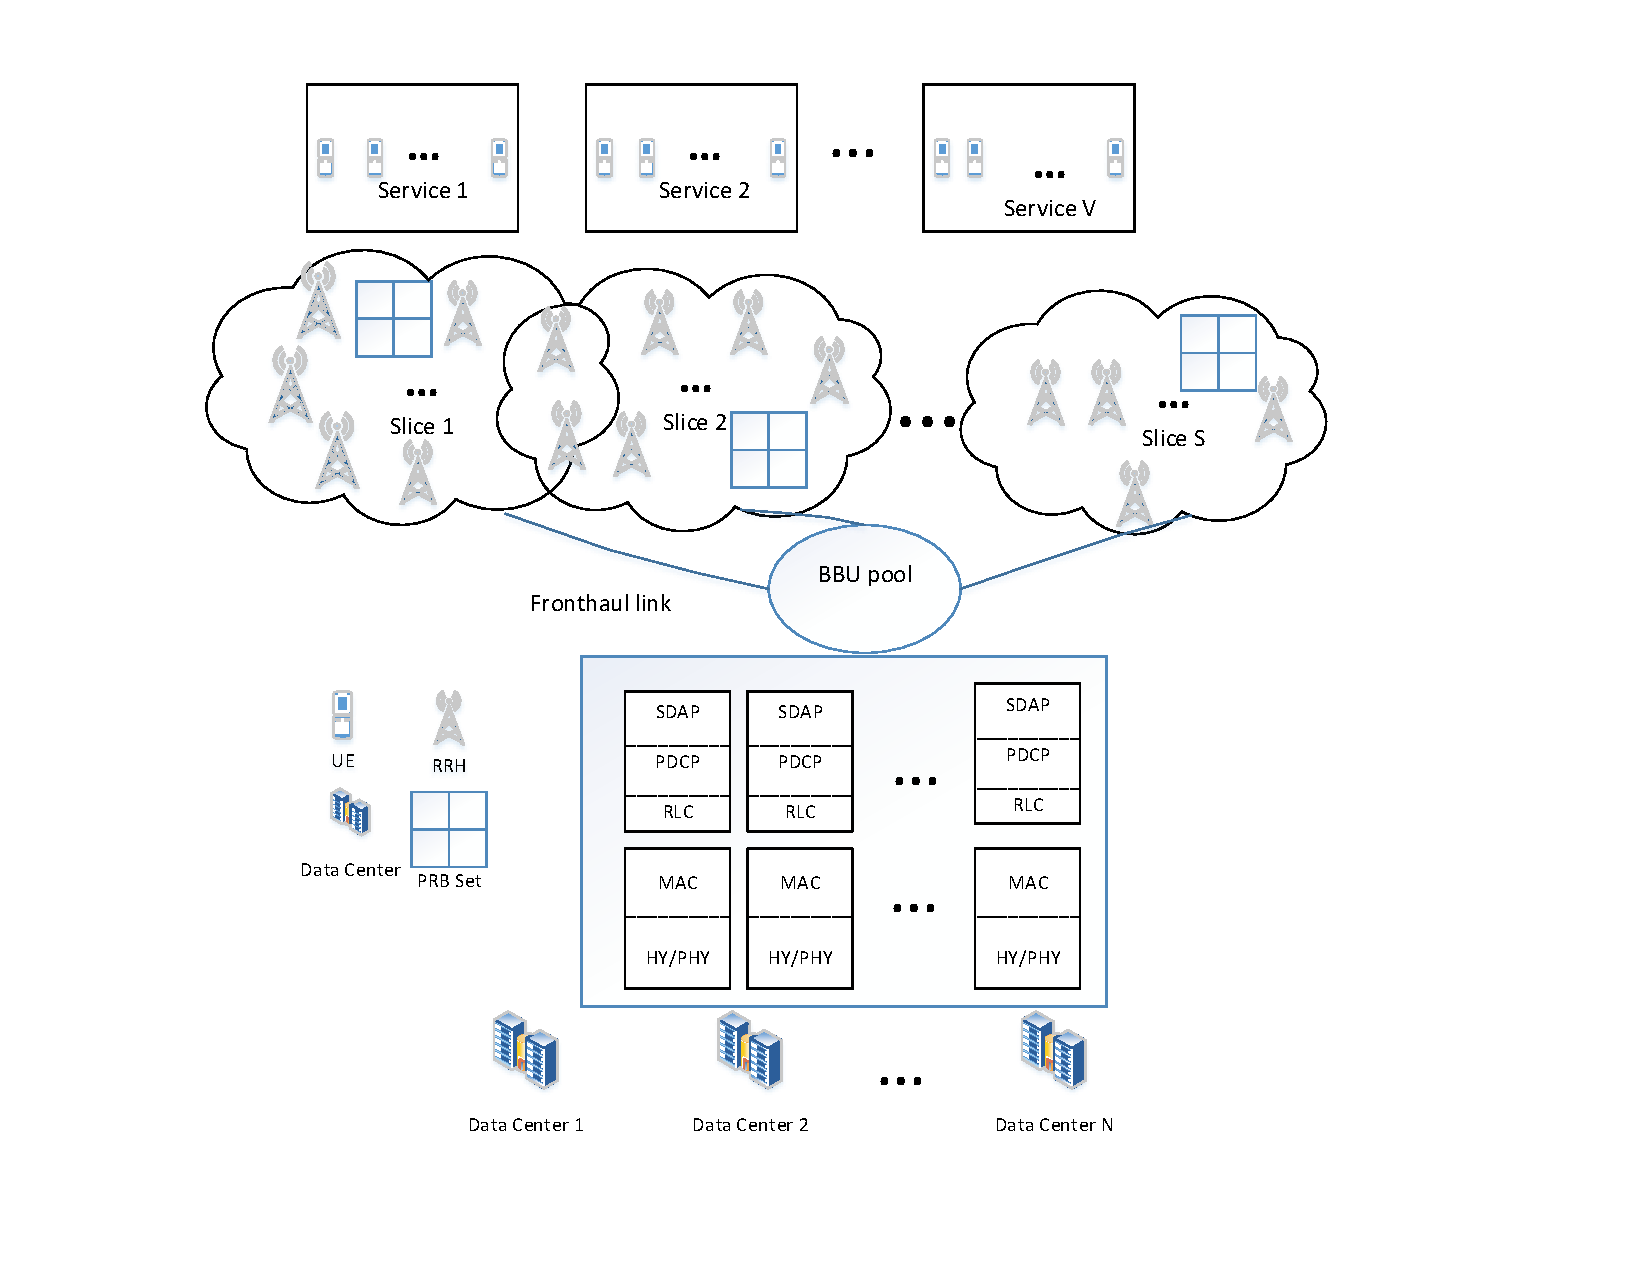
\includegraphics[scale=0.45]{c2}
  \caption{Network sliced O-RAN system}
  \label{fig:c11}
\end{figure} 
Responsibility of wireless systems of the fifth generation covers a wide range types of services. In order to provide the requirement of these services, Network Slicing (NS) is implemented to virtualize the common physical network into several logical end-to-end networks. \newline
To communicate between BBU-pool and RRHs, fronthaul interface which is fiber link is assumed with limited capacity. Compression of message which is passed through these links, is a consequence of limited fronthaul capacity.\\
In BBU-Pool, using cloud-computing, enhance performance of system by virtualizing resources
into virtual machines (VMs).
Each VM has a computing processor which is mapped to Virtual Network Functions (VNFs) which is processed arrival data. Also VNFs are mapped to physical resource through NS technique. \newline
In this paper, in figure \eqref{fig:c11}, the downlink of O-RAN system is assumed. UEs are divided to different groups according to 
their service requirements. Also RAN is decoupled to slices to provide services needs. Optimal power allocation and joint mapping slices to services is applied. In addition, mapping slices to physical resources is considered too.
\section{System Model and Problem Formulation}
In this section, first, we present the downlink (DL) of O-RAN System. Then we obtain achievable rate and delays.
Afterward, the main problem is expressed.
\subsection{System Model}
Suppose that there are $S$ slices Serving $V$ services. Each Service $v\in \{1,2,...,V \} $, consists of $U_v$ single antenna users that require certain service. Each slice $s \in \{1,2,...,S \}$ consists of $R_s$ RRHs and $N_s$ PRBs. All the RRHs in a slice that is mapped to a service, transmit signals to all the UEs in specific service. Each RRH $r \in \{1,2,...,R \}$ is connected to BBU pool via an optical fiber link with limited fronthaul capacity. Also each RRH and PRB can serve more than one slice. It is considered that in BBU, the system has two processing layer consists of $M_1$ homogeneous VMs in first layer and $M_2$ homogeneous VMs in second layer.
\subsection{Achievable Rate}
In this subsection, the Achievable Rate is obtained as below.
The achievable data rate for $i^{th}$ UE in $v^{th}$ service can be written as 
\begin{equation}\label{eq1}
\mathcal{R}_{u(v,i)} = B \log_2({1+ \rho_{u(v,i)}})
\end{equation}
where $B$ is the bandwidth of system and $\rho_{u(v,i)}$ is the SNR of $i^{th}$ UE in $v^{th}$ service which is obtained from 
\begin{equation}\label{eq2}
\rho_{u(v,i)} =  \frac{p_{u(v,i)}\sum_{s=1}^{N_s}|\bold{h}_{R_s,u(v,i)}^H \bold{w}_{R_s,u(v,i)}|^2 a_{vs}}{BN_0 + I_{u(v,i)}}
\end{equation}
Where, $p_{u(v,i)}$ represents the transmitted power allocated by RRHs to $i^{th}$ UE in $v^{th}$ service. Also, 
$\bold{h}_{R_s,u(v,i)} \in \mathbb{C}^{{R}_s}$ is the vector of channel gain of wireless link from RRHs in the $s^{th}$ slice to the $i^{th}$ UE in $v^{th}$ service. In addition, $\bold{w}_{R_s,u(v,i)} \in \mathbb{C}^{{R}_s}$ depicts the the transmit beamforming vector from RRHs in the $s^{th}$ slice to the $i^{th}$ UE in $v^{th}$ service. Moreover, $BN_0$ denotes the power of guassian additive noise and $I_{u(v,i)}$ is the power of interfering signals. 
To obtain SNR as formulated in equation \eqref{eq2}, let $\bold{y}_{U_v}\in \mathbb{C}^{U_v} $ be the received signal's vector of all users in $v^{th}$ service which is given by equation \eqref{eq3}
\begin{equation}\label{eq3}
\bold{y}_{U_v} = \sum_{k=1}^{N_k}\sum_{s = 1}^{N_s} \boldsymbol{H}^H_{\mathcal{R}_s,\mathcal{U}_v}(\boldsymbol{W}_{\mathcal{R}_s,\mathcal{U}_v}\boldsymbol{P}_{U_v}^{\frac{1}{2}}\boldsymbol{x}_{\mathcal{R}_s}+ \boldsymbol{q}_{R_s}) \zeta_{U_v,k,s}+ \boldsymbol{z}_{\mathcal{U}_v}
\end{equation}
where $\boldsymbol{x}_{ \mathcal{R}_s} = [x_{ r_{(s,1)}},...,x_{ r_{(s,\mathcal{R}_s)}}]^T \in \mathbb{C}^{{R}_s } $ depicts the transmitted symbol vector for the $s$-th set of Network slice,  $\boldsymbol{z}_{U_v}$ is the additive Gaussian noise $\boldsymbol{z_{U_v}} \backsim \mathcal{N}(0,N_0\boldsymbol{I}_{{U}_v})$ and $N_0$ is the noise power.
In addition, $\boldsymbol{q}_{R_s} \in \mathbb{C}^{{R}_s }  $ indicates the quantization noise which is made from signal compression in BBU.
\\
Furthermore, $\zeta_{U_v,k,s} \delequal \{\zeta_{u(v,1),k,s},\zeta_{u(v,2),k,s},...,\zeta_{u(v,N_{U_v}),k,s}\}$,
$\zeta_{u(v,i),k,s} \in \{0,1\}$ is a binary parameter that map Physical Resource Blocks (PRB) to UE.
Also as defined before, $\boldsymbol{H}_{\mathcal{R}_s,\mathcal{U}_v}=\left[\boldsymbol{h}_{\mathcal{R}_s,u_{(v,1)}},\ldots,\boldsymbol{h}_{\mathcal{R}_s,v_{(v,\mathcal{U}_v)}}\right]^T  \in \mathbb{C}^{{R}_s\times {U}_v }$ 
shows the channel matrix between RRH set $\mathcal{R}_s$ to UE set
$\mathcal{U}_v$. 
The channel vector from the RRH of  $s^{th}$ slice to the $i^{th}$ UE in the $v^{th}$ service $\boldsymbol{h}_{\mathcal{R}_s,u_{(v,i)}}\in \mathbb{C}^{{R}_s}$ is modeled as below
\begin{equation}
\boldsymbol{h}_{\mathcal{R}_s,u_{(s,i)}} = \boldsymbol{\beta}^\frac{1}{2}_{\mathcal{R}_s,u_{(v,i)}} \boldsymbol{g}_{\mathcal{R}_s,u_{(v,i)}},
\end{equation}
where $\boldsymbol{g}_{\mathcal{R}_s,u_{(v,i)}} \backsim \mathcal{N}(0,N_0\boldsymbol{I}_{\mathcal{U}_v})$ indicates the fast fading and flat fading channel vector and $\boldsymbol{\beta}_{\mathcal{R}_s,u_{(v,i)}}=\text{diag}(b_{r_{(s,1),u_{(v,i)}}},\ldots,b_{r_{(s,\mathcal{R}_s),u_{(v,i)}}})$
represents the large scale fading matrix. Here, it is assumed we have perfect channel state information(CSI).
\\
Moreover, $\boldsymbol{W}_{\mathcal{R}_s,\mathcal{U}_v} = [\boldsymbol{w}_{\mathcal{R}_s,u(v,1)},...,\boldsymbol{w}_{\mathcal{R}_s,u(v,U_v)}] \in \mathbb{C}^{{R}_s\times U_v} $ is the zero forcing beamforming vector to minimize the interference which is indicated as follow
\begin{equation}
\boldsymbol{W}_{\mathcal{R}_s,\mathcal{U}_v} = \boldsymbol{H}_{\mathcal{R}_s,\mathcal{U}_v}(\boldsymbol{H}_{\mathcal{R}_s,\mathcal{U}_v}^H \boldsymbol{H}_{\mathcal{R}_s,\mathcal{U}_v})^{-1}
\end{equation}
Hence, the interference power of $i^{th}$ UE in $v^{th}$ service can be represented as follow
\begin{equation}
\begin{split}
 I_{u_{(v,i)}} &= 
 \underbrace{\sum_{s=1}^{S}\sum_{n=1}^{N_s}\sum_{\substack{l=1 \\ l\neq i}}^{{U}_v} \gamma_{1}  p_{u_{(v,l)}}a_{vs}\zeta_{u_(v,i),n,s}\zeta_{u_(v,l),n,s}}_{\text{(intra-service interference)}}\\
&+ \underbrace{\sum_{\substack{y=1 \\ l\neq v}}^{V}\sum_{s=1}^{S}\sum_{n=1}^{N_s}\sum_{l=1}^{{U}_y} \gamma_{2}  p_{u_{(y,l)}}a_{ys} \zeta_{u_(v,i),n,s}\zeta_{u_(y,l),n,s}}_{\text{(inter-service interference)}}\\
&+\underbrace{ \sum_{s=1}^{S} \sum_{j=1}^{{R}_s} {\sigma_q}_{r_{(s,j)}}^2 |\boldsymbol{h}_{r_{(s,j)}, u_{(v,i)}}|^2 a_{vs}}_{\text{(quantization noise interference)}}.
\end{split}
\end{equation}
where, $\gamma_{1} =|\boldsymbol{h}_{\mathcal{R}_s, u_{(v,i)}}^H \boldsymbol{w}_{\mathcal{R}_{s},u_{(v,l)}}|^2$
and $\gamma_{2} =|\boldsymbol{h}_{\mathcal{R}_s, u_{(v,i)}}^H \boldsymbol{w}_{\mathcal{R}_{s},u_{(y,l)}}|^2$.
It is assumed that interference signal for each UE, is applied from UEs which are using same PRB.
If we replace $p_{u_{(v,l)}}$ and $p_{u_{(y,l)}}$ by $P_{max}$, an upper bound $\bar{I}_{u_{(v,i)}}$ is obtained for $I_{u_{(v,i)}}$. Therefore, $\bar{\mathcal{R}}_{u_{(v,i)}} \forall v , \forall i$ is derived by using $\bar{I}_{u_{(v,i)}}$ instead of $I_{u_{(v,i)}}$ in equation \eqref{eq1} and \eqref{eq2}.\newline
let $\bar{p}_{r_{(s,j)}}$ denote the power of transmitted signal from $j^{th}$ RRH in $s^{th}$ slice.
from equation \eqref{eq3} we have
\begin{equation}
\bar{p}_{r_{(s,j)}} = \sum_{v=1}^{V}\boldsymbol{w}_{r_{(s,j)},\mathcal{U}_{v}} \boldsymbol{P}_{\mathcal{U}_v}^{\frac{1}{2}} \boldsymbol{P}_{\mathcal{U}_v}^{H \frac{1}{2}}   \boldsymbol{w}_{r_{(s,j)},\mathcal{U}_{v}}^H a_{vs} + \sigma_{q_{r(s,j)}}^2.
\end{equation}
As a result the user data capacity on the fronthual link between BBU and the $j^{th}$ RRH in $s^{th}$ slice is formulated as below
\begin{equation}
C_{R_{(s,j)}} = \log{(1+\sum_{v=1}^{V}\frac{w_{r_{(s,j)},\mathcal{D}_{s}} \boldsymbol{P}_{\mathcal{U}_v}^{\frac{1}{2}} \boldsymbol{P}_{\mathcal{U}_v}^{H \frac{1}{2}}   w_{r_{(s,j)},\mathcal{U}_{v}}^H a_{vs}}{ \sigma_{q_{r(s,j)}}^2})},
\end{equation}
\subsection{Mean Delay}
Suppose that we have two processing layer in BBU of O-RAN system. The lower layer is consist of PHY and MAC and the upper layer is consist of RLC, PDCP and SDAP.\newline   
As it is mentioned before, we have $M_1$ VMs in the first layer and $M_2$ VMs in second layer. Each VM in both layers map to one or more slices. So in $s^{th}$ slice, there are $M_{s_1}$ VMs in first layer and $M_{s_2}$ VMs in second layer. Each VM in first and second layer has computational capacity that is  equal to $\mu_1$ and $\mu_2$ respectively. \\
Let the packet arrival of UEs have a Poisson Process with arrival rate $\lambda_{u(v,i)}$ for $i^{th}$ UE in $v^{th}$ service. 
Therefore, the mean arrival data rate of UEs in $s^{th}$ slice in the first layer is 
$\alpha_{s_1} = \sum_{v=1}^{V}\sum_{u=2}^{U_v}a_{vs}\lambda_{u(v,i)}$.  
Furthermore, the mean arrival rate of second layer is approximately equal to the mean arrival rate of first layer $\alpha_{s} =\alpha_{s_1} \approx \alpha_{s_2}$ since, by using Burke’s Theorem, the arrival packets of second layer which is processed in first layer is still Poisson with rate $\alpha_{s}$. 
It is assumed that there are dispatchers in each layer for each slice to divide the incoming traffic to VMs.
Suppose the baseband processing of each VM is depicted as a M/M/1 processing queue.
Each packet is routed by one of VMs of slices. So the mean delay of slice $s$ which is related to incoming traffic rate routed to
each VM in first layer can be written as follow
\begin{equation}
d_{s_1} = \frac{1}{\mu_1 - \alpha_{s}/{M_{s_1}}}
\end{equation}
Also, the delay in $s^{th}$ slice in second layer can be formulated as below
\begin{equation}
d_{s_2} = \frac{1}{\mu_2 - \alpha_{s}/{M_{s_2}}}
\end{equation}
In addition, the arrival data rate to the queue of wireless transmission
 is equal to the arrival data rate of dispatcher.
Moreover, it is assumed that the service time of transmission queue for each slice $s$ has 
 an exponential distribution with mean $1/(R_{{tot}_s})$ and can be modeled as a M/M/1 queue. Therefore, 
the mean delay of transmission layer is 
\begin{equation}
d_{s_{tr}} = \frac{1}{R_{{tot}_s} - \alpha_{s}}
\end{equation}
Where, $R_{{tot}_s} =  \sum_{v=1}^{V}\sum_{u=2}^{U_v}a_{vs}R_{u(v,i)}$.
We define a new parameter which indicates mean delay of each slice
\begin{equation}
D_{s} = d_{s_1} + d_{s_2} + d_{s_{tr}} \forall s
\end{equation} 
\subsection{Physical Resource}
Assume each VM is mapped to one virtual network function (VNF) for simplicity. Each VNF requires
physical resources which contain RAM, Memory and CPU.
Let, the required resources for VNF $f$ in slice $s$ is represented by a three dimensional vector as follow
\begin{equation}
\bar{\Omega}_{(f,s)} = \{\Omega_{R_{f,s}}, \Omega_{M_{f,s}}, \Omega_{C_{f,s}} \}
\end{equation} 
Where,$\bar{\Omega}_{(f,s)}\in \mathbb{C}^{3}$ and $\Omega_{R_{f,s}}, \Omega_{M_{f,s}}, \Omega_{C_{f,s}}$ indicate the amount of required RAM, Memory and CPU.
Moreover total amount of required RAM, Memory and CPU of all VNFs in a slice is a three dimension vector which is defined as
\begin{equation}
\bar{\Omega}_{s}^{tot} = \sum_{f=1}^{F_s}\bar{\Omega}_{(f,s)}
\end{equation}
Where, $F_s = M_{s_1} + M_{s_2}$ is the total number of VNFs in slice $s$.
\newline
Also, in the Core Network (CN), there are $D_c$ data centers (DC), which served VNFs. Each DC contains several servers that supply VNF's needs.
The amount of RAM, Memory and CPU is denoted respectively by $\tau_{R_{j}}, \tau_{M_{j}}$ and $\tau_{C_{j}} $ for $j^{th}$ DC.
\begin{equation*}
\tau_j = \{\tau_{R_{j}}, \tau_{M_{j}}, \tau_{C_{j}} \}
\end{equation*}
Also we define a weighted parameter of $\tau_j$ as follow
\begin{equation}\label{wt}
\begin{split}
\hat{\Omega}_{s}^{tot} &= w_R \bar{\Omega}_{R_s}^{tot} + w_M \bar{\Omega}_{M_s}^{tot} + w_C \bar{\Omega}_{C_s}^{tot} \\
\hat{\tau}_j &= w_R \tau_{R_{j}} + w_M \tau_{M_{j}} + w_C \tau_{C_{j}}
\end{split}
\end{equation}
Where, $\boldsymbol{w} = \{w_R, w_M, w_C\}$ are the weight of RAM, Memory and CPU.
\subsection{Problem Statement}
One of the most important parameters to estimate the optimality of the system is energy efficiency which is represented as sum-rate to sum-power as follow
\begin{equation}
\eta(\boldsymbol{P},\boldsymbol{A}) := \frac{\sum\limits_{v=1}^{V} \sum\limits_{k=1}^{{U}_v}\mathcal{R}_{u_{(v,k)}} }{\sum\limits_{s=1}^{S} \sum\limits_{i=1}^{{R}_s}\bar{p}_{r_{(s,i)}}} = \frac{\mathfrak{R}_{tot}(\boldsymbol{P},\boldsymbol{A})}{P_{r_{tot}}(\boldsymbol{P},\boldsymbol{A})},
\end{equation}
Assume the power consumption of baseband processing at each data center that is mapped to VNFs of a slice is depicted as
$\phi$. So the total power can be represented as  
\begin{equation*}
\phi_{tot} = \sum_{s=1}^{S}\sum_{d=1}^{D_c}y_{s,d}\phi
\end{equation*} 
Where, $y_{s,d}$ is a binary variable which indicates whether $d^{th}$ data-center is mapped to VNFs of $s^{th}$ slice or not.\\
In this paper, the main goal is to simultaneously maximize sum-rate and minimize sum-power with the presence of constraints which is written as follow, 
\begin{subequations}
\begin{alignat}{4}
\max\limits_{\boldsymbol{P}, \boldsymbol{A}, \boldsymbol{Y} }   \quad &   \eta(\boldsymbol{P},\boldsymbol{A})+\frac{1}{\phi_{tot}(\boldsymbol{Y})} \\
\text{subject to} \quad  & \bar{p}_{r_{(s,i)}} \leq P_{max} && \quad \forall s, \forall i, 
 \label{c11} \\
&p_{u_{(v,k)}}  \geq 0  &&\quad \forall v, \forall k,\label{c12} \\
&\mathcal{R}_{u_{(v,k)}} \geq  \mathcal{R}_{u_{(v,k)}}^{min} && \quad \forall v, \forall k,\label{c13} \\                                 
&C_{r_{(s,i)}} \leq C_{r_{(s,i)}}^{max}  &&\quad \forall s, \forall i, \label{c14}\\
&D_{s} \leq D_{s}^{max}  &&\quad \forall s,\label{c15} \\
& \sum_{s=1}^{S}a_{vs} \geq 1 &&\quad \forall s, \label{c21} \\
& \sum_{d=1}^{D_c}\sum_{v=1}^{V}y_{s,d}a_{vs} \geq 1\times\sum_{v=1}^{V}a_{vs} &&\quad \forall s,\label{c23} \\
& \bar{\Omega}_{\mathfrak{z}(s)}^{tot} = \sum_{f=1}^{F_s}\bar{\Omega}_{\mathfrak{z}(f,s)} \leq  \sum_{d=1}^{D_c} y_{s,d} \tau_{\mathfrak{z}_d}                      
 && \quad \forall \mathfrak{z}, \forall s  \label{c22}
\end{alignat}
\label{constraints}
\end{subequations}
Where,$\boldsymbol{P} =[p_{u(v,k)}]  \forall v , \forall k $, $\boldsymbol{A} =[a_{vs}]  \forall v , \forall s $ and $\boldsymbol{Y} =[y_{s,d}]  \forall s , \forall d $. 
Equation \eqref{c11}, \eqref{c12} indicates respectively that the power of each RRH do not exceed the maximum power and power of each UE is a positive integer value. Also \eqref{c13} shows that the rate of each UE is more than a threshold. \eqref{c14} and \eqref{c15} depicts respectively that the capacity of fronthaul link is limited and the delay of receiving signal should be less than a threshold.  
Furthermore, \eqref{c21}
ensure that each service is mapped to one or more slice.
Also, \eqref{c23} guarantee that each slice (VNFs in two layers of slice) has been placed to one or more physical resources (DC). Moreover, in \eqref{c22}  $\mathfrak{z}\in \{M,R,C\}$, which supports 
that we have enough physical resource for VNFs of each slice.\newline 
The main optimizaiton problem which is formulated as \eqref{constraints} can be decomposed into two independent optimization problem A and B. The problem A is introduced as bellow
\begin{subequations}
\begin{alignat}{4}
\max\limits_{\boldsymbol{P}, \boldsymbol{A} }   \quad &   \eta(\boldsymbol{P},\boldsymbol{A})\\
\text{subject to} \quad  & \bar{p}_{r_{(s,i)}} \leq P_{max} && \quad \forall s, \forall i,   \\
&p_{u_{(v,k)}}  \geq 0  &&\quad \forall v, \forall k, \\
&\mathcal{R}_{u_{(v,k)}} \geq  \mathcal{R}_{u_{(v,k)}}^{min} && \quad \forall v, \forall k, \\                                 
&C_{r_{(s,i)}} \leq C_{r_{(s,i)}}^{max}  &&\quad \forall s, \forall i,\label{cc14} \\
&D_{s} \leq D_{s}^{max}  &&\quad \forall s, \label{cc15} \\
& \sum_{s=1}^{S}a_{vs} \geq 1 &&\quad \forall s
\end{alignat} 
\label{constraints1}
\end{subequations}
and the problem B is 
\begin{subequations}
\begin{alignat}{4}
\min\limits_{\boldsymbol{y} }   \quad &   \phi_{tot}(\boldsymbol{Y})\\
\text{subject to} \quad & \sum_{d=1}^{D_c}\sum_{v=1}^{V}y_{s,d}a_{vs} \geq 1\times\sum_{v=1}^{V}a_{vs} &&\quad \forall s, \\
&  \bar{\Omega}_{\mathfrak{z}(s)}^{tot} = \sum_{f=1}^{F_s}\bar{\Omega}_{\mathfrak{z}(f,s)} \leq  \sum_{d=1}^{D_c} y_{s,d} \tau_{\mathfrak{z}_d}                      
 && \quad \forall \mathfrak{z}, \forall s\label{eqomega}
\end{alignat}
\label{constraints2}
\end{subequations}
\section{Proposed Method For Problem \eqref{constraints1}}
In this subsection, the proposed method is applied to solve the optimization problem.
We want to solve \eqref{constraints1}. Since the problem is non-convex and NP-Hard iterative algorithm is applied.
To solve the problem and obtain optimum $\boldsymbol{A}$ and $\boldsymbol{P}$ we divide problem \eqref{constraints1} to 
two different part that can be solved iteratively.  
\subsection{First Part of Sub-Problem A}\label{firstsub}
Firstly, we need to obtain $\boldsymbol{A}$ by fixing $\boldsymbol{P}$ in the problem \eqref{constraints1} and updating this parameter at the end of each iteration. Two different method is applied to acquire $\boldsymbol{A}$. The first method is using MOSEK and second method is a heuristic algorithm.
The details of heuristic algorithm are represented in \textbf{Algorithm} \eqref{alg}.  
\begin{algorithm}
\caption{Mapping Slice to Service}\label{alg}
\begin{algorithmic}[1]
\State Sort services according to their priority, the number of UEs in it and their requirements in descending order.
\State Sort slices according to the number of PRBs, RRHs and VNFs in two layers and the Capacity of their resources in descending order. 
\For {$i \gets 1$ to $S$}
\For {$j \gets 1$ to $V$}
\State Set $a_{ij} = 1$
\State Obtain Parameters of System
\If {conditions \eqref{c11}, \eqref{c12}, \eqref{c13} and \eqref{c14} is not applied} 
\State Set $a_{ij} = 0$;
\Else
\State break from inner loop;
\EndIf 
\State \textbf{end if}
\EndFor 
\State \textbf{end for}
\EndFor 
\State \textbf{end for}
\end{algorithmic}
\end{algorithm}
\subsection{Second Part of Sub-Problem A}\label{secondsub}
In this part, by assuming that $\boldsymbol{A}$ is fixed, the optimal power of UEs in each service is achieved.
\begin{theorem}\label{t2}
 $\eta^*$ which is the optimum energy efficiency can be achieved if
\begin{equation}\label{q2}
\begin{split}
&\max \limits_{\boldsymbol{P}} (\mathfrak{R}_{tot}(\boldsymbol{P}) - \eta^* P_{r_{tot}}(\boldsymbol{P}))=\\
& \mathfrak{R}_{tot}(\boldsymbol{P}^*) - \eta^* P_{r_{tot}}(\boldsymbol{P}^*) =0.
\end{split}
\end{equation}
\end{theorem}
\begin{proof}
See Appendix A
\end{proof}
The second subproblem can  be solved using Lagrangian function and iterative algorithm. 
Since, Interference is a function of power of UEs, for simplicity, we assume an upper bound $\bar{I}_{u_{(v,i)}}$ for interference (the worst-case). 
In order to make equation \eqref{constraints1} as a standard form of convex optimization problem, it is required to change the variable of equations \eqref{cc14} and \eqref{cc15}.
Lagrangian function is written as follow
\begin{equation}\label{lagrang}
\begin{split}
\mathcal{L}(\boldsymbol{P}; \boldsymbol{\lambda}, \boldsymbol{\mu}, \boldsymbol{ \xi}, \boldsymbol{ \kappa}) & = \sum\limits_{v=1}^{V} \sum\limits_{k=1}^{U_v}\mathcal{\bar{R}}_{u_{(v,k)}} 
- \eta \sum\limits_{v=1}^{V} \sum\limits_{i=1}^{\mathcal{R}_s}\bar{p}_{r_{(s,i)}}\\
&+\sum\limits_{s=1}^{S} \sum\limits_{k=1}^{U_v} \lambda_{u_{(v,k)}} (\mathcal{\bar{R}}_{d_{(s,k)}}-\mathcal{R}_{u_{(v,k)}}^{max})\\
&- \sum\limits_{s=1}^{S} \sum\limits_{i=1}^{R_s} \mu_{r_{(s,i)}} (\bar{p}_{r_{(s,i)}}-P_{max})\\
&- \sum\limits_{s=1}^{S} \sum\limits_{i=1}^{R_s} \xi_{r_{(s,i)}} (\bar{p}_{r_{(s,i)}}-\sigma_{q_{r(s,j)}}^2 2^{C_{r_{(s,i)}}^{max}}).\\ 
&+ \sum\limits_{v=1}^{V} \sum\limits_{k=1}^{U_v} \kappa_{u_{(v,k)}} \sum\limits_{s=1}^{S}(R_{u_{(v,k)}} -\mathfrak{D_s})a_{vs}.\\ 
\end{split}
\end{equation}
Where,$\mathfrak{D_s}=\frac{1}{D_{s}^{max}-d_{s_1}-d_{s_2}}+\alpha_s$. Also, $\boldsymbol{\lambda}$, $\boldsymbol{\mu}$, $\boldsymbol{\xi}$ and $\boldsymbol{ \kappa}$ are the matrix of Lagrangian multipliers which have non-zero positive elements. Optimal power is obtained from equation \eqref{lagrang} as follow
\begin{equation}
p_{u(v,i)}^{*} = \frac{\mathfrak{y}_{u(v,i)}\mathfrak{w}_{u(v,i)}-\mathfrak{x}_{u(v,i)}\mathfrak{z}_{u(v,i)}}{\mathfrak{x}_{u(v,i)}\mathfrak{w}_{u(v,i)} }
\end{equation}
where, $\mathfrak{y}_{u(v,i)}= (-\mu_{u(v,i)}+\lambda_{u(v,i)}+\kappa_{u_{(v,k)}}+1)\frac{B}{Ln_2}$ and 
$\mathfrak{w}_{u(v,i)} = \sum_{s=1}^{N_s}|\bold{h}_{R_s,u(v,i)}^H \bold{w}_{R_s,u(v,i)}|^2 a_{vs}$. Also 
$\mathfrak{z}_{u(v,i)} = BN_0 + \bar{I}_{u(v,i)}$ and $\mathfrak{x}_{u(v,i)} = \sum\limits_{s=1}^{S} \sum\limits_{i=1}^{R_s} (\xi_{r_{(s,i)}}+\eta)||w_{r_{(s,j)},u_{(v,i)}}||^2$. 
By using sub-gradient method, the optimal power $\boldsymbol{P}$ is obtained. 
%\section*{References}
\subsection{Solving two part of Sub-problem A iteratively}
In \eqref{firstsub} and \eqref{secondsub} the details of solving each part of subproblem is depicted. 
Here, the algorithm of solving sub-problem A is shown in \textbf{Algorithm} \eqref{alg2}
\begin{algorithm}
\caption{Joint Network Slicing and Power Allocation}\label{alg2}
\begin{algorithmic}[1]
\State Set the maximum number of iterations $I_{max}$, convergence condition $\epsilon_{\eta}$  and the initial value $\eta^{(1)} = 0$
\State Set $\boldsymbol{P} = \boldsymbol{P}_{max}$
\For {$counter \gets 1$ to $I_{max}$}
\State Achieve $\boldsymbol{A}$ by applying Algorithm \eqref{alg}
\State Obtain $\boldsymbol{P}$ by using sub-gradient method which is mentioned in \eqref{secondsub}.
\If {$ \mathfrak{R}_{tot}(\boldsymbol{P}^{(i)},\boldsymbol{A}^{(i)}) - \eta^{(i)} P_{r_{tot}}(\boldsymbol{P}^{(i)},\boldsymbol{A}^{(i)}) < \epsilon_{\eta} $} 
\State Set $\boldsymbol{P}^*= \boldsymbol{P}^{(i)} $, $\boldsymbol{A}^*= \boldsymbol{A}^{(i)} $   and  $ \eta^{*} =\eta^{(i)} $;
\State break;
\Else
\State $i= i+1$, Setting $\boldsymbol{P} = \boldsymbol{P}^{(i)}$ ;
\EndIf 
\State \textbf{end if}
\EndFor 
\State \textbf{end for}
\end{algorithmic}
\end{algorithm}
\subsection{Sub-Problem B}
In this subsection, we want to solve equation \eqref{constraints2} which is the placement of virtual resources to physical resource in order to minimize the number of using DCs. 
To achieve optimum $\boldsymbol{Y}$ heuristic algorithm and Mosek is applied. The details of heuristic algorithm is written in \textbf{Algorithm} \eqref{alg3}. In this algorithm, if a slice does not admit to a specific DC, it is remain for next placement. In next placement the residual slices, map to more than one DC according to their requirements.
\begin{algorithm}
\caption{Plecement of Physical resources into Virtual resources}\label{alg3}
\begin{algorithmic}[1]
\State Sort Slices according to $\hat{\Omega}_{s}^{tot} , \forall s$ in descending order.
\State Sort DCs according to $\hat{\tau}_j , \forall j$ in descending order. 
\State $\boldsymbol{Y} = \boldsymbol{0}$
\For {$d \gets 1$ to $D_c$}
\For {$s \gets 1$ to $S$}
\If {$\sum_{d=1}^{D_c}y_{s,d}==0$ and $\bar{\Omega}_{\mathfrak{z}(s)}^{tot} \leq \tau_{\mathfrak{z}_j} \forall \mathfrak{z}, \forall s$  } 
\State Set $y_{s,d} = 1$;
\State {$\tau_j$ $\gets$ {$\tau_j - \bar{\Omega}_{s}^{tot}$}}
\EndIf 
\State \textbf{end if}
\EndFor 
\State \textbf{end for}
\EndFor 
\State \textbf{end for}
\State  $\{ind_{residual} = s|({\sum_{d=1}^{D_c}y_{s,d}==0})\}$
\State Sort residual amount of DCs same as before in descending order.
\State Sort residual slices same as before in descending order.
\For {$r \gets 1$ to $S_{residual}$}
\For {$n \gets 1$ to $D_c$}
\State Set $y_{s,d} = 1$;
\State {$\bar{\Omega}_{s}^{tot}$ $\gets$ {$\bar{\Omega}_{s}^{tot}- \tau_j$}}
\If {$\bar{\Omega}_{s}^{tot}==0$}
\State Set $y_{s,d} = 1$;
\State {$\tau_j$ $\gets$ {$\tau_j - \bar{\Omega}_{s}^{tot}$}}
\State {break inner loop}
\EndIf 
\State \textbf{end if}
\EndFor 
\State \textbf{end for}
\EndFor 
\State \textbf{end for}
\end{algorithmic}
\end{algorithm}
\section{Simulation}
In this section, Simulation and numerical results for the main problem are depicted.
\bibliographystyle{ieeetr}
\bibliography{ref}
\end{document}
